%%%%%%%%%%%%%%%%%%%%%%%%%%%%%%%%
\section{Introduction}
%%%%%%%%%%%%%%%%%%%%%%%%%%%%%%%%

% bugs allow access to data/code outside of the current module
Modern software systems are complex but monolithic, 
comprising multiple interacting subsystems,
incorporating third-party code like libraries, plugins, or interpreted code,
while interacting over untrusted 
interfaces including networks, shared memory, file systems, or user input.
The lack of isolation between the components of a monolithic program 
allows vulnerabilities to have far-reaching consequences.
An attacker who exploits one component can corrupt other parts ---
for example, a buggy Linux driver can compromise
core kernel data structures.
The traditional process abstraction for running monolithic software
violates the Principle of Least Privilege~\cite{SaltzerS75}
which requires components to only have access to the data necessary
for their operation.
Instead, all code running within a process' address space has 
equal permissions to all data and code regions
allowing attackers to subvert pre-defined interfaces between components.
For example, calls between components can jump to an arbitrary address
bypassing checks on function call arguments.

% compartmentalization enables least privilege
Intra-address space compartmentalization allows developers to 
\emph{isolate components} of a program within compartments, 
only granting each compartment permissions to access their own data.
When compromised, a buggy component cannot access another
component's data.
Conversely, a component is guaranteed integrity of its private
data against other corrupted compartments.
Compartmentalization is a key defense mechanism that leverages the 
inherent modularity of code to 
fortify the cloud~\cite{v8isolates,ShillakerP20,miller2021} and 
desktop~\cite{fffission} sandboxed environments, 
programs with third-party libraries~\cite{GhosnKPLB21}%,ZimmermannSTP19}, % VasilakisKRDDS18, 
and underpins the design of security-focused microkernel operating
systems~\cite{RozierAABGGHKLLN88, Hildebrand92, LevinCCPW75, GolubDFR90}.
Compartmentalization constrains the negative effects of the myriad possible faults 
in software, 
including memory safety violations and logic errors, 
to compartment boundaries.
For example, the Log4Shell exploit (CVE-2021-44228~\cite{cve202144228}) which
allowed attackers to exfiltrate secrets and inject arbitrary code in
memory-safe programs can be mitigated by isolating the vulnerable Log4j framework
in a separate compartment.

% properties of a good compartmentalization mechanism
The compartmentalization mechanism enforcing
the rules of access and communication between the program's 
components must be secure, performant and flexible.
To be secure, the mechanism must enforce policy-dependent 
restrictions on memory accesses and inter-compartment calls
in the face of powerful attackers.
Particularly, the mechanism must prevent compromised compartments
from escalating their memory access rights or from bypassing
inter-compartment call gates.
%
Developers for performance- and security-critical software such as
operating systems constantly trade off the benefits of protection mechanisms
against their overheads.
The mechanism must implement low overhead checks and operations to support 
fine-grained compartmentalization for such programs.
Faster compartment switching, for example, 
enables developers to refactor programs into smaller compartments
with more frequent compartment switches,
improving security while maintaining the same performance.
%
Finally, a flexible mechanism which is able to support the wide variety of 
desired compartmentalization policies will bolster developer adoption.

% why existing mechanisms are insufficient
Existing compartmentalization mechanisms lack one or more 
desirable features, often trading security for performance,
or flexibility for backward compatibility or implementation simplicity.
Traditional, process-based 
isolation~\cite{KleinEHACDEEKNSTW09,LittonVE0BD16,WitchelCA02MMP}
only permits costly, microsecond-scale compartment switches.
On the other end of the spectrum, protection-key~\cite{guide2011intel} based 
mechanisms~\cite{ParkLXMK19,ERIMOberwagner19,SchrammelWSS0MG20Donky}
are performant, with nanosecond-scale switches,
but fail to deter attackers with code-injection capabilities.
Mechanisms co-locating permissions with page-based virtual 
memory~\cite{ERIMOberwagner19,SchrammelWSS0MG20Donky,LeeSK18,DuHXZC19XPC,
KoningCBGA17,HedayatiGJCSSM19Hodor}
improve compatibility with existing page-tables but
inherit the limited reach of modern 
Translation Lookaside Buffers (TLBs), incurring overheads
for programs with large working sets.
Finally, other mechanisms~\cite{KoningCBGA17,FrassettoJLS18} 
target simpler policies, 
such as protecting a single trusted compartment from an untrusted 
compartment.

\seccells achieves the trifecta of secure, flexible, and high-performance 
compartmentalization by embedding compartmentalization into the 
architectural virtual memory abstraction.
\seccells proposes 
\begin{inparaenum}[\itshape i\upshape)]
\item \emph{TCB-maintained VMA-scale} access control, and 
\item unprivileged (i.e., userspace) instructions implementing 
\emph{securely-bounded} compartmentalization primitives, with
\item software implementing call gates, call stacks, and context isolation.
\end{inparaenum}
Related efforts towards languages, compilers and libraries for
compartmentalization can extend these benefits to developers
by using \seccells as the underlying isolation mechanism.

For the first pillar, access control, \seccells introduces the 
first VMA-granular permissions table consolidating permissions for
all compartments into a single data structure designed for
efficient permission lookups.
In contrast, previous mechanisms use per-compartment permission tables 
with either duplicate VMA bounds information~\cite{WitchelCA02MMP},
duplicate per-page permissions within a 
VMA~\cite{ERIMOberwagner19,SchrammelWSS0MG20Donky},
or both~\cite{DuHXZC19XPC,LittonVE0BD16}.
Deduplicating VMA bounds accelerates compartment switching, eliminating
the need to re-load bounds for the target compartment.
VMA-scale permission tracking requires smaller VMA-based permission
lookaside buffers while also overcoming TLB-reach limits.

For the second pillar, 
\seccells accelerates common compartmentalization operations with
novel, low-cost unprivileged instructions.
Particularly, \seccells is the first mechanism to
allow generic, unprivileged permission transfer from userspace.
\seccells maintains the integrity of permissions by bounding 
the semantics of untrusted userspace operations to known-safe parameters --- 
the hardware checks the compartment switch instruction to enforce call gates,
and permission transfer instructions to prevent privilege escalation.

\seccells' final pillar leverages the flexibility of software for 
operations where possible without compromising security or 
performance (context isolation, call gates and call stack maintenance).
\seccells{} shows the first software mechanism for restoring register context
following a compartment switch, necessary for isolating compartment contexts,
without trusting any general-purpose registers.

In this chapter, we:
\begin{itemize}
  \item define \seccells' key security and performance objectives
        and survey how related mechanisms meet these goals,
  \item propose \seccells, a novel, secure, flexible, and performant 
        mechanism which introduces compartments 
        into the architectural virtual memory abstraction,
  \item apply \seccells to typical application scenarios,
  \item present a hardware implementation of \seccells based on the 
        5-stage in-order RISC-V RocketChip, and
  \item characterize \seccells' performance for compartmentalizing
        micro- and macro-benchmarks.
\end{itemize}

%%%%%%%%%%%%%%%%%%%%%%%%%%%%%%%%
\section{Background}
\label{sec:background}
%%%%%%%%%%%%%%%%%%%%%%%%%%%%%%%%

\subsection{Principles supporting Compartmentalization}

\paragraph{Modularity and Principle of Least Privilege}
Explaining modularity.
\begin{itemize}
  \item Modularity is a key principle in modern software design
  \item Modularity helps handle exploding code complexity, simplifies design
  \item Modules are clustered around separate functionality
  \item Modularity lends itself to extensibility - code sharing relies on modularity
  \item Modules force developers to think of, and implement interfaces
  \item Modularity lends itself to PoLP: modules don't need access to everything
\end{itemize}

Explaining PoLP.
\begin{itemize}
  \item Principle of Least Privilege recommends that principals only have
        the minimal access (do data or other resources) required to perform
        their functionality
  \item Implies complicated programs should be further decomposed
  \item Modularity simplifies decomposition, we already have logical parts
  \item PoLP extends to compartments within a program.
  \item PoLP should be temporal too (privileges last only as long as required)
  \item PoLP helps mitigate bugs. A bug is not able to access as much data or stuff.
  \item PoLP forces interfaces, and enables checks at these interfaces
\end{itemize}

\subsection{Isolation and Communication}

A program cannot execute entirely with isolated compartments.
Compartments need to coordinate to get the job done, i.e., compartments need
to request work from other compartments.

Compartments have interfaces, from which other compartments can request work.
This means there will be control flow between compartments.

For improved security, compartmentalization requires isolation of resources.
Typically, this requires - 
\begin{itemize}
  \item Isolation in memory. Memory access needs to be restricted according to
        the policy. This allows compartments to have private data, or to
        share data between a specific set of compartments.
  \item Isolation in control flow. Restrictions on which compartment can call
        which other compartment. 
        For example, sandboxed code should only be able to call into the
        runtime compartment, not directly other sandboxes or to supervisor.
  \item Isolation in system resources, such as file descriptors, semaphores
        and threads. 
        Particularly useful in Linux, where all resources are described as
        files, and file descriptors are used ubiquitously for system resources.

\end{itemize}

%%%%%%%%%%%%%%%%%%%%%%%%%%%%%%%%
\section{Objectives For Architectural Isolation}
% \section{The case for a novel compartmentalization mechanism}
\label{sec:reqs}
%%%%%%%%%%%%%%%%%%%%%%%%%%%%%%%%

Compartmentalization mechanisms are characterized by a specific set of 
objectives, which we introduce in this section.
We demonstrate how \seccells' objectives benefit compartmentalization
using two representative programs described below and
discuss how alternate goals lead to the differing designs
of related mechanisms.

The characteristics of a compartmentalization mechanism 
determine its applicability.
Primarily, the mechanism must be \emph{secure} (\req{1}) 
and enforce the
restrictions on data access and communication despite arbitrarily compromised
compartments. 
Second, the mechanism must be \emph{performant} (\req{2}), 
with low overhead for enforcing its checks and restrictions.
A performant mechanism allows high-performance software
to be compartmentalized without violating performance targets.
Finally, a mechanism must be \emph{flexible} (\req{3}) in order to 
support the varying needs of software across security and 
performance criticality, and their corresponding isolation policies.
A flexible mechanism does not make additional assumptions such as
a hierarchical trust structure among compartments, and allows
data to be shared in an arbitrary fashion.
We concretize these objectives, based on insights from existing
and candidate compartmentalized programs and related work, 
in the following subsections.
We justify each objectives' importance using the
two characteristic programs described below.

\begin{figure}
  \centering
  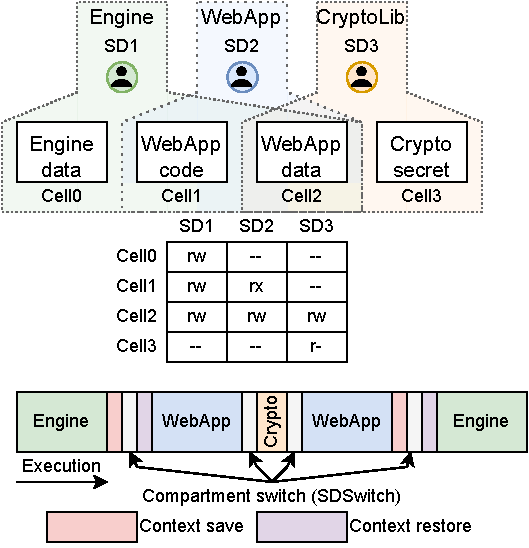
\includegraphics[width=0.65\linewidth]{media/seccells/browser_webapp.pdf}
  \caption{Browser compartmentalization with three compartments.}
  \label{fig:browser_eg}
  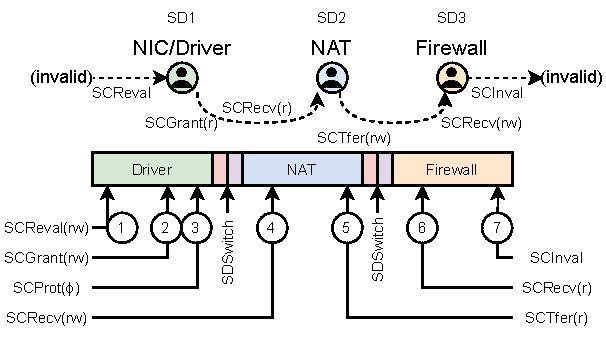
\includegraphics[width=\linewidth]{media/seccells/dataflow_app.pdf}
  \caption[Permission transfers for a packet between \seccells compartments.]
          {Permission transfers for a packet between \seccells compartments. 
            The figure shows the compartment executing the relevant \seccells 
            instructions on one core.}
  \label{fig:dataflow_app}
  %\Description[<short description>]{<long description>}
\end{figure}

\paragraph{Use case: Browser}
The first program, a browser (\autoref{fig:browser_eg}), consists of
a just-in-time (JIT) compilation engine (Engine), 
a sandboxed web application (WebApp) compiled and executed by the Engine, and 
a cryptographic library (CryptoLib) storing a secret key for encryption.
The compartmentalization policy aims to isolate the Engine's data
and CryptoLib's secret from the possibly malicious WebApp.
Borrowing the threat model for browsers, we assume that the 
WebApp can exploit bugs in the Engine's compiler to 
generate and execute arbitrary code as the WebApp compartment,
ultimately aiming to leak the browser's data or the cryptographic secret.
The developer aims to prevent unauthorized inter-compartment data accesses
by enforcing the per-compartment permissions shown in the figure.
To maintain similar performance to the monolithic version, the developer
desires minimal overhead from operations added due to compartmentalization:
context switching and compartment switching.

\paragraph{Use case: Network Function Virtualization}
The second program is a virtual network function pipeline 
(\autoref{fig:dataflow_app}) consisting of three stages progressively
performing processing steps on a stream of packets.
In particular, this pipeline has three compartmentalized stages, 
implementing the network card driver (Driver) which
generates packets, 
a network address translation (NAT) stage which translates IP 
addresses in the header based on a translation table, and
a firewall stage that implements checks on the packet headers
based on a rule table.
In this example, we omit further stages for simplicity.
Middleboxes in datacenters and the internet~\cite{MartinsAROHBH14}
commonly contain virtual network functions sharing a buffer pool
in uncompartmentalized dataflow pipelines.
Translation and rule tables in the NAT and Firewall compartments
must be isolated in private regions, protecting them from potential bugs 
in the Driver compartment that processes input from untrusted traffic 
from external sources.
The programmer requires isolation of network stages for high reliability
of the middlebox and low cost for passing packets between stages for 
line-rate packet processing, enabled by zero-copy packet flow 
through permission transfer.


%-------------------------------
\subsection{Threat Model}
\label{sec:reqs:threat}
%-------------------------------

Our threat model assumes an attacker who wants to compromise a 
compartmentalized program with multiple communicating compartments.
We assume that the attacker has compromised one or more compartments, and
gained the ability to both generate arbitrary code and execute it,
but is restricted to the compromised compartments.
The attacker wishes to compromise confidentiality, integrity, or 
gain code execution in other compartments.
%
For example, the attacker might try to:
% \begin{inparaitem} for an inlined bullet point list instead
\begin{itemize}
  \item gain permissions and directly access (load/store) 
        another compartment's private memory,
  \item inject unsolicited code/data regions in another 
        compartment's memory,
  \item execute unintended code in another compartment,
  \item create new compartments, or
  \item achieve any combination of the above.
\end{itemize}

The policy used for compartmentalization is assumed to be sound, and the software
implementations of the modules comprising compartments are assumed to be
free of bugs that can be exploited via only their exposed communication
interfaces.
\seccells' trusted computing base (TCB) consists of the hardware implementation
and the supervisor.
Exploitable bugs in the policy or TCB can lead to a compromise irrespective of the
compartmentalization mechanism.
While speculative side-channel attacks are outside the scope of our threat model,
we discuss \seccells' speculative resiliency in \autoref{sec:seccells:discussion}.

%-------------------------------
\subsection{Security Objectives}
\label{sec:reqs:security}
%-------------------------------
A secure mechanism must enforce restrictions on a compartmentalized program,
as described below.

\paragraph{Obj. \req{1a}}
Mechanisms must implement \emph{access control},
validating every memory access against the policy.
For the browser in \autoref{fig:browser_eg}, the table
holds policy-defined permissions for each compartment and memory region.
Mechanisms must, for example, prevent all accesses by the compromised
WebApp from reading the Engine or CryptoLib's private regions as per the
policy.
Mechanisms must also prevent corruption of policy-defined permissions
stored in memory or registers.
Intel MPK-based protection~\cite{ParkLXMK19}, for example, loads
permissions from a user-controlled register when executing a
\Code{wrpkru} instruction, allowing a compartment to corrupt its 
own permissions.

\paragraph{Obj. \req{1b}}
Inter-compartment communication consisting of cross-compartment calls 
demand \emph{validity checks}.
Relevant validity checks include checking that 
\begin{inparaenum}[\itshape i\upshape)]
  \item the entry point is valid,
  \item the calling compartment is allowed to call the target compartment, 
  \item the return respects the call stack, and
  \item the passed arguments are valid.
\end{inparaenum}
Compartment switches from the WebApp to the Engine must use valid entry
points which are followed by argument-validating code. Failure to enforce this
constraint enables
control-flow attacks such as return-oriented programming (ROP).
Vanilla Intel MPK-based protection also lacks such entry-point checks
to accompany \Code{wrpkru} instructions.

\paragraph{Obj. \req{1c}}
\emph{Context isolation} accompanying a cross-compartment call is 
essential for protecting mutually distrusting compartments.
After a cross-compartment call, the callee compartment (for example, the Engine) 
must be able to fetch its context without trusting the registers which
are controlled by the caller (correspondingly, the WebApp), 
representing an attack vector.
The WebApp, for example, could try to switch to the Engine with a malicious stack pointer
register, attempting to corrupt the Engine by reading from the wrong stack.
CODOM~\cite{VilanovaBNEV14}, for example, assumes a migrating thread model
and is vulnerable to attacks through an invalid register state.

\paragraph{Obj. \req{1d}}
Mechanisms that allow untrusted compartments to modify or transfer their 
permissions must prevent privilege escalation %~\cite{ZeldovichBKM06} 
through \emph{TCB-imposed limitations} on these operations.
Specifically, compartments should only be allowed to surrender access 
permissions or transfer existing permissions to other compartments.
A stage in the network function pipeline, for example, should not be allowed
to grant write permissions for a packet to the next stage if it has
read-only permissions.
Transferring permissions between compartments must also be mutual, requiring
explicit actions from both compartments.
One-directional permission transfers studied by 
Lipton~\textit{et. al.}~\cite{LiptonS77} 
allow compartments to either steal other compartments'
permissions (violating confidentiality) or
inject illegal data or code into other compartments (violating integrity).
Linux, which allows processes to specify their own permissions
when \Code{mmap}ing shared regions, violates this objective without 
syscall mechanisms like SECCOMP.

\paragraph{Obj. \req{1e}} 
\emph{Temporary exclusive access} to otherwise 
shared data regions enables compartments to use data regions safely,
preventing exploitation of double-fetches.
With exclusive access to a packet, the Firewall stage of the network function
pipeline can safely validate and use addresses in the packet header in-place 
(without copying), with the assurance that another corrupt stage cannot
concurrently modify the packet.
XPC~\cite{DuHXZC19XPC} recognizes this objective, allowing exclusive access
to a single region tracked by the Relay Segment register.

\paragraph{Obj. \req{1f}} 
\emph{Auditability}, the ability to easily determine the 
global access permissions, facilitates auditing compliance to a 
compartmentalization policy by checking which compartments have access to
which memory region.
A browser might regularly audit its permissions to ensure that the WebApp
has not escalated its privileges.
An audit for a mechanism with a centralized permissions store, 
such as page tables, must only check this store simplifying audits.
In contrast, an audit for CHERI~\cite{WatsonWNMACDDGL15} requires an 
expensive, full-memory scan since the set of memory regions accessible to a
compartment is the transitive closure of capabilities held in its registers,
along with capabilities held in any memory region accessible through these 
registers.

%-------------------------------
\subsection{Performance Objectives}
\label{sec:reqs:performance}
%-------------------------------
Low-overhead checks and operations allow performance-critical
programs to be compartmentalized.

\paragraph{Obj. \req{2a}} 
\emph{Single-cycle access verification} in the common case
is essential for core throughput.
While most mechanisms meet this objective in the best (not common) case, 
page-table based isolation mechanisms suffer from the limited scalability
of Translation Lookaside Buffers (TLBs) used to cache permissions.
Programs with large datasets can incur high TLB miss rates, with 
correspondingly high verification latency in the common case due to 
page-table walks.
UNIX process-based protection particularly suffers from this limitation since
modern Address Space ID (ASID)-tagged TLBs will effectively contain duplicate
entries for a shared page with separate permission for each compartment,
effectively dividing an already capacity-limited structure among 
compartments~\cite{HsuHEP16}.
This objective implicitly requires the mechanism to support
a sufficiently large number of compartments and data regions.
A mechanism with small limits, like Intel MPK which is restricted to
16 colors for data regions, will incur overheads from software workarounds
required to virtualize the corresponding resource~\cite{ParkLXMK19}.

\paragraph{Obj. \req{2b}} 
Cross-compartment calls are essential and
frequent for communication between fine-grained compartments
necessitating \emph{fast compartment switches}.
Fine-grained library isolation~\cite{GhosnKPLB21} requires compartment 
switches accompanying every function call to an untrusted library.
A program isolating short-running functions, 
such as AES encryption using hardware AES-NI extensions, 
can incur a compartment switch every tens or hundreds of 
cycles~\cite{AbdAllahAES}.
Specialized hardware instructions accessible from userspace are
essential for cheap compartment switches in tens of cycles.
Even the fastest supervisor-mediated compartment switch still costs
hundreds of cycles~\cite{WatsonWNMACDDGL15}.

\paragraph{Obj. \req{2c}}
\emph{Fast, zero-copy permission transfer} enables programs to 
efficiently move data between compartments.
Data copying for passing large buffers during 
compartment calls can overwhelm high-performance programs, 
such as our example network function pipeline.
Such applications typically pass packets by reference between 
unisolated stages profiting from zero-copy.
Cheap permission transfers, within ten to hundred cycles, enable 
such applications to be compartmentalized with performance
comparable to the monolithic versions.
UNIX process-based permission transfers instead involve microsecond-scale
system calls, precluding their use for practical compartmentalization.

%-------------------------------
\subsection{Flexibility}
\label{sec:reqs:flexibility}
%-------------------------------

A mechanism demands flexibility to be suitable
to compartmentalization across a variety of application domains. 

\paragraph{Obj. \req{3a}}
For flexibility, a mechanism must support \emph{arbitrary sharing of data
regions},
requiring independent per-compartment per-region permissions.
A private region, for example, should be accessible by only a single
compartment.
Another shared region might allow read access to one compartment, 
write access to another, and execute permissions to a third.
Mechanisms that target hierarchical security, for example, limit
flexibility --- the trusted  compartment implicitly has permission
to access an untrusted compartment's data --- and exclude wide 
applicability.
In contrast, even if the WebApp in the browser trusts the Engine,
the Engine is denied execute permissions to the WebApp's code.
A mechanism must support, but not be exclusive to, specific trust
models such as nested compartments.

\paragraph{Obj. \req{3b}}
To scale performance overheads with security objectives, we
introduce a desirable property, \emph{security-proportionality}.
A security-proportional mechanism allows policies to trade-off 
overheads for security when unnecessary.
Despite not trusting the WebApp, transitions from the WebApp to
CryptoLib can elide context switching required for register 
isolation under a specific condition.
Verification approaches~\cite{KolosickNJWLGJS22Verizero,ChenRSL16} 
can be used to prove that a small function in CryptoLib does not leak the key
under the assumption that entry points are enforced,
and that the function's code overwrites registers used to store the key 
before returning to the WebApp.
By using the cheaper migrating thread model~\cite{FordL94},
a security-proportional mechanism can reduce overheads where acceptable.
Process-based isolation, for example, is not security-proportional
since every compartment switch incurs the same non-negotiable overheads 
(including context switching, page-table switching, or scheduling).

%-------------------------------
\subsection{Alternate Visions for Compartmentalization}
\label{sec:reqs:related}
%-------------------------------

% Text for the camera ready. Reinstate.
\seccells envisions a future where the mechanism supports 
widespread application
compartmentalization efforts, with consequently differing goals
and designs compared to related mechanisms.
% \seccells targets different goals compared to related mechanisms
% consequently resulting in drastically differing designs.
% 
First, some mechanisms only support \emph{custom-tailored use cases}
such as differentiating between single trusted-untrusted 
compartments~\cite{HedayatiGJCSSM19Hodor,KoningCBGA17,Kilpatrick03}, % ,MogosanuRD18
or a binary classification of data as (in)sensitive~\cite{FrassettoJLS18}.
CODOMs~\cite{VilanovaBNEV14} link code addresses to compartments,
restricting code sharing that is abundant in modern programming.
Specialization allows simpler hardware mechanisms, but do not support
a broad spectrum of applications.
Second, \seccells does not aim to compartmentalize existing software with
zero-modifications.
While automated isolation techniques provide a crucial first step towards
compartmentalized programs~\cite{RoesslerAPMPKPB21,KirthDCLDGNVF22,
VasilakisKRDDS17}, security-critical software requires refactoring to fully
realize the benefits of proper compartmentalization.
Finally, related works target \emph{compatibility with legacy hardware}
or existing or upcoming software/hardware mechanisms and abstractions for 
isolation.
Numerous mechanisms try to compartmentalize using process-based isolation
implemented by the OS~\cite{LittonVE0BD16,DuHXZC19XPC,KleinEHACDEEKNSTW09}, 
retrofitting compartmentalization onto an abstraction originally designed for
multiprogramming on unicore processors.
Others leverage Intel MPK~\cite{HedayatiGJCSSM19Hodor,ERIMOberwagner19,KoningCBGA17}
or similar protection-key based mechanisms~\cite{SchrammelWSS0MG20Donky},
synergizing with traditional page table-based virtual memory.
Targeting immediate adoption, Hodor~\cite{HedayatiGJCSSM19Hodor} and 
LOTRx86~\cite{LeeSK18} (ab)used existing processor features intended for 
other purposes to isolate compartments.
HAKC~\cite{mckee2022preventing} leverages state-of-the-art ARM extensions, 
PAC and MTE, to compartmentalize the Linux kernel, but requires a two-level 
clustering of closely-connected compartments to overcome MTE's 
compartment scaling limitations and still incurs a significant performance hit.
With the sole exception of Mondrian~\cite{WitchelCA02MMP}, proposals
assume current page-based virtual memory.
Meanwhile, trends in applications and memory architectures have led to a 
resurgence in range-based translations and protections among academic 
proposals~\cite{BasuGCHS13,YanLNB19,PhamVJB12,0003BOBFP21midgard,KarakostasGACHM15}
and commercial processors including AMD's Zen lineup~\cite{preservingvma}.
\autoref{tab:req_comparison} summarizes the objectives satisfied by related 
mechanisms (justification in Appendix~\ref{app:justification_table1}).
We discuss related mechanisms further in \autoref{sec:related}.
 
% Camera ready TODO: Should I make figure and table styles consistent?
% If yes, follow the procedure described here
% https://tex.stackexchange.com/questions/166814/table-caption-in-uppercase-i-dont-know-why
\begin{table}
  \centering
  \caption[Qualitative comparison of compartmentalization mechanisms]
          {Comparison of compartmentalization mechanisms based on 
          compliance with the objectives described in \autoref{sec:reqs}.
          Limited compliance is marked with ``$\sim$''.
          }
% \begin{tabular}{l | c c c c c c | c c c | c c |}
  \begin{tabular}{l | c@{\hspace{1em}} c@{\hspace{1em}} c@{\hspace{1em}} c@{\hspace{1em}} c@{\hspace{1em}} c@{\hspace{1em}} | c@{\hspace{1em}} c@{\hspace{1em}} c@{\hspace{1em}} | c@{\hspace{1em}} c@{\hspace{1em}} |}
    \toprule
              & \multicolumn{6}{c|}{\req{1}}                  & \multicolumn{3}{c|}{\req{2}} & \multicolumn{2}{c|}{\req{3}} \\
              & a     & b     & c     & d     & e     & f     & a     & b     & c     & a     & b             \\ \midrule
  UNIX        & \yes  & \yes  & \yes  & N/A   &       & \yes  &       &       &       & \yes  &               \\
  Mondrian    & \yes  & \yes  & \yes  & N/A   &       & \yes  & \yes  &       &       & \yes  &               \\
  lwC         & \yes  & \yes  & \yes  & N/A   &       & \yes  &       &       &       & \yes  &               \\
  CODOM       & \yes  & \yes  &       & N/A   &       & \yes  &       & \yes  &       &       & \yes          \\
  XPC         & \yes  & \yes  & \yes  & \yes  & \yes  & \yes  &       & \yes  & $\sim$& \yes  &               \\
  MPK         &       &       &       &       &       & $\sim$&       & \yes  & \yes  & \yes  & \yes          \\
  ERIM        & $\sim$& $\sim$&       &       &       & $\sim$&       & \yes  & \yes  & \yes  & \yes          \\
  Donky       & $\sim$& \yes  &       & N/A   &       & \yes  &       & \yes  & \yes  & \yes  &               \\
  CHERI       & \yes  & \yes  & \yes  &       &       &       &       &       & \yes  & \yes  &               \\
  \seccells   & \yes  & \yes  & \yes  & \yes  & \yes  & \yes  & \yes  & \yes  & \yes  & \yes  & \yes          \\ \bottomrule
  \end{tabular}
  \label{tab:req_comparison}
\end{table}

\paragraph{Complementary requirements}
To satisfy application requirements,
programs compartmentalized with \seccells' mechanisms require
complementary properties from other parts of the system
including secure compartmentalization policies, 
a secure and performant supervisor interface, 
and formal verification of application-level properties
aided by programming conventions.
For example, supervisors might include a syscall for 
microsecond-scale compartment creation~\cite{LittonVE0BD16}.
Safe calling conventions can provide formal guarantees against
inadvertent information leakage from the stack~\cite{SkorstengaardDB20}.
These investigations are outside the scope of this thesis.

\paragraph{\seccells overview}
\seccells is a compartmentalization mechanism designed
to satisfy the above objectives across a wide array of 
programs, providing flexibility and performance without compromising on 
security.
\seccells stores permissions in a centralized permissions table accessible 
only by the supervisor and hardware.
A novel, range-based memory management unit (MMU) and 
lookaside buffer design (\autoref{sec:seccells:design:access_ctl})
allows single-cycle access control on the fast path satisfying 
objectives \req{1a}, \req{1f}, \req{2a}, and \req{3a}.
\seccells introduces fast, userspace instructions for common 
compartmentalization operations (see \autoref{tab:seccell_ops}): 
switching compartments, transferring permissions and validating
exclusive access for data regions (\autoref{sec:seccells:design:instructions}).
These instructions satisfy requirements \req{1b}, \req{1e},
\req{2b}, \req{2c}.
\seccells delegates context isolation, call-stack maintenance,
and argument validation to software.
\autoref{sec:seccells:design:softmech} outlines how software can
securely and efficiently implement context isolation and call-stack 
maintenance.
Software implementing these functions satisfy security (\req{1b}, \req{1c})
and flexibility (\req{3a}, \req{3b}) objectives.

%%%%%%%%%%%%%%%%%%%%%%%%%%%%%%%%
\section{\seccells}
\label{sec:seccells:design}
%%%%%%%%%%%%%%%%%%%%%%%%%%%%%%%%

\begin{figure}
  \centering
  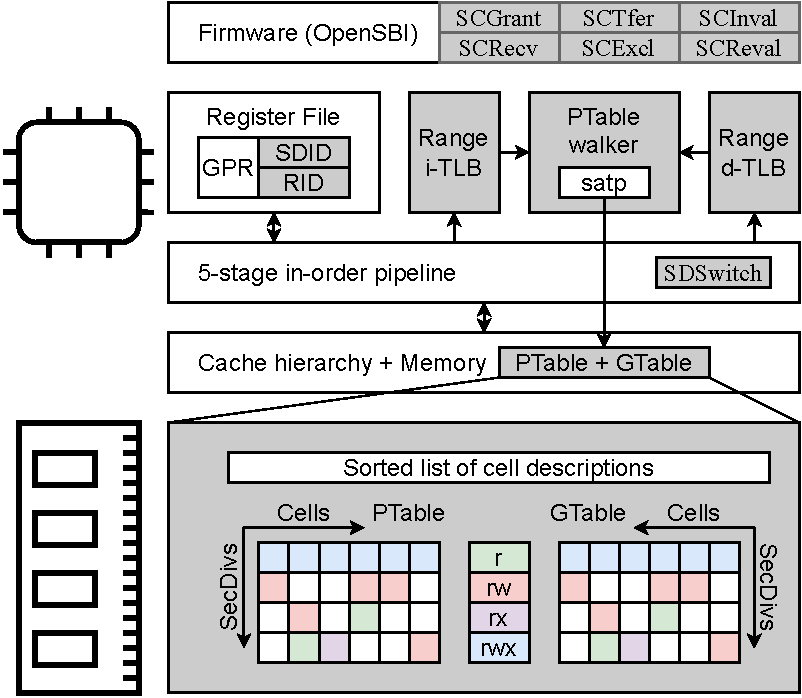
\includegraphics[width=0.85\linewidth]{media/seccells/seccell_arch.pdf}
  \caption[\seccells: Architecture.]
          {\seccells' architecture, highlighting modified hw/sw in gray.}
  \label{fig:seccell_arch}
  %\Description[<short description>]{<long description>}
\end{figure}

\seccells proposes hardware-software co-design to satisfy the
manifold objectives for efficient and secure compartmentalization.
The key insight that \emph{compartmentalization operations from untrusted userspace
are secure with TCB-maintained permission checks} allows \seccells to
implement compartment switch and permission transfer through
trusted hardware-checked userspace instructions which are
hundred to thousand times faster compared to traditional supervisor calls.
Pragmatically, \seccells retains software for operations such as 
context switching which, while common, would not benefit significantly 
from hardware support.
Software implementations of such operations achieve higher flexibility and
resilience to implementation errors at negligible or low additional performance
cost compared to a hardware implementation.
% Hardware compartment switching eliminates generic supervisor-dependent 
% overheads due to system call dispatch, scheduling and resource accounting, 
% as well as an extra context switch and pipeline serialization for entering
% the kernel.
For example, both hardware and software context switching can saturate
the L1 data cache bandwidth, achieving similar performance.
The second insight is that VMA-based permission tracking eliminates 
permission duplication inherent in page-table entries for pages 
within a VMA.
\seccells leverages this insight, eliminating overheads for 
permission storage (compared to equivalent page tables) and 
allowing hundred-times smaller core-side lookaside buffers. 

\seccells protects compartments, application-defined mutually untrusting
parts of a program, by controlling their access to memory regions.
Each compartment is allocated a Security Division (\secdiv)
with individual permissions to each VMA-granularity data region (\cell{}).
The Browser (\autoref{fig:browser_eg}), for example, has 
three compartments (Engine, WebApp and CryptoLib) allocated 
\secdivx{1}-\secdivx{3}, and four \cell{}s.
\seccells augments each core with a read-only register (\sid) tracking 
the currently executing compartment.
Along with a table for storing permissions (\ptable) and a modified
MMU for enforcing the permissions, \seccells implements single-cycle
access control.
The WebApp \secdiv has executable permissions
to one code \cell and read-write permission to one data \cell.
Userspace instructions (see \autoref{tab:seccell_ops}) enable 
secure compartment switching and permission surrender/transfer.
% For implementation reasons regarding how risc-v wants to use ecalls to enter
% the kernel, we must make urid writable by the kernel in our prototype.
% In a pure seccells world, where sdswitches are used for syscalls, we
% might no longer need writable urid (caveat switching programs).
%
% Mat: we could argue that privileged world can always write/override but this
% may be too implementation specific
Another per-core read-only register (\rid) tracks the caller after a 
compartment switch, allowing the callee to securely identify 
its caller.
% \andres{Not sure if this argument is enough, we can use a memory
% segment for that and rely on a compartmentalization policy (memory segment not
% writable by the callee). Is the performance argument sufficient?}
% Atri: Not sure how that would work
During permissions transfer, a granted permissions table (\gtable) tracks
outstanding permissions.
Further, the design implements context isolation and secure call stacks
in software leveraging the above hardware primitives.
\autoref{fig:seccell_arch} summarizes \seccells's architecture.
The detailed layout of cell descriptors, the \ptable, and the \gtable 
are shown in Appendix~\ref{app:ptable}.


%-------------------------------
\subsection{Access control}
\label{sec:seccells:design:access_ctl}
%-------------------------------
The Permissions Table (\ptable) stores 
per-cell, per-\secdiv permissions for the compartmentalized 
program.
For each \cell, the permissions for each \secdiv are independent
and define the degree of sharing for that \cell.
Compartment-private data stores allow only one \secdiv non-null 
permissions in this table.
Shared \cell{}s can be readable, writable, or executable by more than one
\secdiv.
For a JIT compiler, the \cell holding generated data will be writable
by the compiler \secdiv, while being executable by the sandboxed code's
\secdiv.
The \ptable is stored in privileged supervisor memory, restricting
accesses (including stores) from userspace.
\autoref{fig:browser_eg} shows the permissions for the three browser 
compartments, assigned to separate \secdiv{}s, to the four 
data regions, similarly assigned to \cell{}s.
\seccells' current \ptable design supports a large number of 
\secdiv{}s and \cell{}s ($2^{29}$ and $2^{32}$ respectively), 
vastly exceeding application requirements.
A finely-compartmentalized modern browser, for example, will only require
a few hundred compartments, isolating each loaded shared 
library (around 100 on the author's Firefox installation)
and per-tab rendering compartments~\cite{barth2008security}.

\seccells replaces the core's MMU with a \ptable walker and 
range-based lookaside buffers for permissions and translations.
The MMU checks access permissions based on the accessed address and
the executing \secdiv identified by the core's \sid register.
The lookaside buffers track a small number of frequently accessed
\cell{}s, along with \sid-tagged permissions.
In the common case, access control verifies permissions from
entries in this buffer.
When accesses miss in this buffer, the \ptable walker reads the
required permission from the \ptable.
The walker first performs a (fast) binary search in a sorted list of permissions
to find the correct cell containing the accessed address, then
reads the correct permission from the \ptable for that cell.
The location of the permission in the \ptable is found through very 
simple arithmetic.

\seccells' \ptable layout and MMU design has three
key advantages: fast \ptable walks, scalability to large data 
working sets, and low silicon cost.
The \ptable layout aids fast permission lookups by
sorting the \cell descriptors, allowing a binary search
for the \cell descriptor containing an address, 
and the contiguous layout of the permissions for a particular
\secdiv, which improves spatial locality for \ptable walks.
Range-based lookaside buffers also enable scalability for
programs with large datasets, since permissions should be 
verified against TLB entries in the common case.
With growing dataset sizes, traditional processors require larger 
TLBs in order to track additional page translations and permissions.
Importantly, all permissions for pages within a VMA are
the same, leading to duplication in TLB entries' permissions.
However, the growth of program datasets has exceeded the
TLB reach of modern processors, leading to attempts at 
range-based translations (explicitly managed by the 
supervisor~\cite{YanLNB19}, or implicitly through 
coalescing~\cite{PhamVJB12}).
In contrast, as dataset sizes grow, the \cell count remains 
constant and the size of \cell{}s increases.
Previous work in range-based translation caching~\cite{YanLNB19,0003BOBFP21midgard} 
have also demonstrated that 
processors require hundred-times smaller range-based lookaside buffers 
than in traditional systems, drastically reducing silicon cost.
Research proposals~\cite{0003BOBFP21midgard, ZhangSRL10} 
have also tackled
external fragmentation from range-based translations 
by introducing a system-wide page table after the
last-level cache.

%-------------------------------
\subsection{Userspace Instructions}
\label{sec:seccells:design:instructions}
%-------------------------------

\begin{table}[]
  \centering
  \caption{Overview of \seccells' userspace instructions.}
  \begin{tabular}{l | l}
    \toprule
    Instruction & Purpose                                           \\
    \midrule
    \sdswitch   & Switch to another \secdiv                         \\
    \scprot     & Change current \secdiv{}'s permission to \cell    \\
    \scinval    & Mark a \cell invalid                              \\
    \screval    & Revalidate an invalid \cell                       \\
    \scgrant    & Grant \cell permissions to another \secdiv        \\
    \screcv     & Accept granted \cell permissions                  \\
    \sctfer     & Grant and drop \cell permissions                  \\
    \scexcl     & Check for exclusive access to a \cell             \\
    \bottomrule
  \end{tabular}
  \label{tab:seccell_ops}
\end{table}

\begin{figure*}[!t]
  \vspace{-1\baselineskip}
  \rule{\textwidth}{1pt}
  \centering
  \textbf{\seccells Program State\\}
  \vspace{-0.5\baselineskip}
  \rule{\textwidth}{1pt}
  \vspace{-2\baselineskip}
  \begin{multicols}{2}
    \begin{algorithmic}[1]
      \State $S$ = Set of $M$ \secdiv{}s incl. supervisor $SD_{sup}$
      \State $C$ = Set of $N$ cells, each valid or invalid
      \State Per-core register $SID$
      \State Per-core register $RID$
      \State \ptable $PT: S \times C \mapsto \mathscr{P}(\set{r, w, x})$
      \State \gtable $GT: S \times C \mapsto S \times \mathscr{P}(\set{r, w, x})$
    \end{algorithmic}
  \end{multicols}
  \vspace{-1.4\baselineskip}
  \rule{\textwidth}{1pt}

\vspace{-0.7\baselineskip}
\begin{multicols}{2}
\removelatexerror

    % General notation:
    % c_i         for a cell
    % SD_j        for a secdiv
    % p_{i,j}     for PT(SDj,ci)
    % gp_{tgt}    for GT perms

    % SDSwitch algorithm
    \begin{algorithm}[H]
      \caption{SDSwitch($addr$, $SD_{tgt}$) \\
        Switch to $SD_{tgt}$ at instruction pointer $addr$   }
        \begin{algorithmic}[1]

          \State $c_i \gets cell(addr)$
          \State \textbf{assert} $valid(c_i)$

          \State \textbf{assert} instruction at $addr$ is $SDEntry$
          \State \textbf{assert} $x \in PT(SD_{tgt}, c_i)$
          \State instruction pointer $\gets addr$
          \State $RID \gets SID$
          \State $SID \gets SD_{tgt}$
        \end{algorithmic}
        \label{alg:sdswitch}
    \end{algorithm}
    \vspace{-0.5\baselineskip}

    % SCProtect algorithm
    \begin{algorithm}[H]
      \caption{SCProt($addr$, $perm$) \\
      Restrict rights to $addr$ to $perm$              }
      \begin{algorithmic}[1]

        \State $c_i \gets cell(addr)$
        \State \textbf{assert} $valid(c_i)$

        \State $p_{i,cur} \gets PT(SD_{cur}, c_i) $
        \State \textbf{assert} $perm \subseteq p_{i,cur}$

        \State $PT(SD_{cur}, c_i) \gets perm$
      \end{algorithmic}
      \label{alg:scprotect}
    \end{algorithm}
    \vspace{-0.5\baselineskip}

    % SCGrant algorithm
    \begin{algorithm}[H]
      \caption{SCGrant($addr$, $SD_{tgt}$, $perm$) \\
      Grant $SD_{tgt}$ $perm$ rights to $addr$             }
      \begin{algorithmic}[1]

        \State $c_i \gets cell(addr)$
        \State \textbf{assert} $valid(c_i) \land perm \ne \phi$

        \State $p_{i,cur} \gets PT(SD_{cur}, c_i)$
        \State \textbf{assert} $perm \subseteq p_{i,cur}$

        \State $GT(SD_{cur}, c_i) \gets (SD_{tgt}, p_{tgt})$
      \end{algorithmic}
      \label{alg:scgrant}
    \end{algorithm}
    \vspace{-0.5\baselineskip}

    % SCRecv algorithm
    \begin{algorithm}[H]
      \caption{SCRecv($addr$, $SD_{src}$, $perm$) \\
      Accept $perm$ rights to $addr$ from $SD_{src}$      }
      \begin{algorithmic}[1]

        \State $c_i \gets cell(addr)$
        \State \textbf{assert} $valid(c_i) \land perm \ne \phi$

        \State $(SD_{tgt}, gp_{tgt}) \gets GT(SD_{src}, c_i)$
        \State $p_{i,cur} \gets PT(SD_{cur}, c_i)$
        \State \textbf{assert} $SD_{cur} = SD_{tgt} \land perm \subseteq gp_{tgt}$

        \If{$perm = gp_{tgt}$}
          \State $GT(SD_{src}, c_i) \gets (SD_{inv}, \phi)$
        \Else
          \State $GT(SD_{src}, c_i) \gets (SD_{tgt}, gp_{tgt} - perm)$
        \EndIf
        \State $PT(SD_{cur}, c_i) \gets perm \cup p_{i, cur} $

      \end{algorithmic}
      \label{alg:screcv}
    \end{algorithm}
    \vspace{-\baselineskip}

    % SCTfer algorithm
    \begin{algorithm}[H]
      \caption{SCTfer ($addr$, $SD_{tgt}$, $perm$) \\
      Transfer all $perm$ rights for $addr$ to $SD_{tgt}$    }
      \begin{algorithmic}[1]
        \State SCGrant($addr$, $SD_{tgt}$, $perm$)
        \State SCProtect ($addr$, $\phi$)
      \end{algorithmic}
      \label{alg:tfer}
    \end{algorithm}
    \vspace{-1.5\baselineskip}

    % SCReval algorithm
    \begin{algorithm}[H]
      \caption{SCReval($addr$, $perm$)  \\
      Re-validate address $addr$ with $perm$ rights}
      \begin{algorithmic}[1]

        \State $c_i \gets cell(addr)$
        \State \textbf{assert} $invalid(c_i) \land perm \ne \phi$

        \State Validate $c_i$
        \State $PT(SD_{cur}, c_i) \gets perm$

      \end{algorithmic}
      \label{alg:screval}
    \end{algorithm}
    \vspace{-1.5\baselineskip}

    % SCInval algorithm
    \begin{algorithm}[H]
      \caption{SCInval($addr$)  \\
      Invalidate $addr$ cell}
      \begin{algorithmic}[1]

        \State $c_i \gets cell(addr)$
        \State \textbf{assert} $valid(c_i)$

        \ForAll{$SD_j \in S - \set{SD_{sup}, SD_{cur}}$}
          \State $p_{i, j} \gets PT(SD_j, c_i)$
          \State $(SD_{tgt}, gp_{tgt}) \gets GT(SD_j, c_i)$
          \State \textbf{assert} $p_{i,j} = \phi \land gp_{tgt} = \phi \land SD_{tgt} = SD_{inv}$
        \EndFor

        \State $PT(SD_{src}, c_i) \gets \phi$
        \State $GT(SD_{cur}, c_i) \gets (SD_{inv}, \phi)$

        \State Invalidate $c_i$
      \end{algorithmic}
      \label{alg:scinval}
    \end{algorithm}
    \vspace{-1.5\baselineskip}

    % SCExcl algorithm
    \begin{algorithm}[H]
      \caption{SCExcl($addr$, $perm$) \\
      Verify exclusive $perm$ rights to $addr$       }
      \begin{algorithmic}[1]

        \State $c_i \gets cell(addr)$
        \State \textbf{assert} $valid(c_i) \land perm \ne \phi$

        \State $p_{i,cur} \gets PT(SD_{cur}, c_i) $
        \State \textbf{assert} $perm \subseteq p_{i,cur}$

        \State $ (SD_{tgt}, gp_{tgt}) \gets GT(SD_{cur}, c_i)$
        \If{$ perm \cap gp_{tgt} \neq \phi$}
          \State \textbf{return} $False$
        \EndIf

        \State $excl \gets True$
        \ForAll{$SD_j \in S - \set{SD_{sup}, SD_{cur}}$}
          \State $p_{i,j} \gets PT(SD_j, c_i)$
          \State $(SD_{tgt}, gp_{tgt}) \gets GT(SD_j, c_i)$
          \If{$ perm \cap p_{i,j} \neq \phi \lor perm \cap gp_{tgt} \neq \phi$}
            \State $excl \gets False$
          \EndIf
        \EndFor
        \State \textbf{return} $excl$
      \end{algorithmic}
      \label{alg:sccount}
    \end{algorithm}
    \vspace{-\baselineskip}
  \end{multicols}

  \caption{\seccells' state and userspace instructions.}
  \label{fig:seccell_ops_formal}
\end{figure*}


\seccells introduces 8 new serializing userspace instructions for
accelerating common compartmentalization operations 
(\autoref{tab:seccell_ops}).
These instructions, formally defined in \autoref{fig:seccell_ops_formal}, 
implement speculation-free compartment switching with 
checked entry points, permission surrender and transfer for zero-copy dataflow.

The \sdswitch instruction targets secure, 
low-overhead compartment switching within userspace.
\sdswitch resembles function call instructions, with 
direct and indirect variants, additionally switching the
core's \sid register and saving the caller's \sid to \rid.
Since the \sid register is not writable from userspace, 
inter-compartment calls must use \sdswitch.
The cost of executing an \sdswitch is essentially the
cost of pipeline serialization, plus the negligible cost
of updating core registers, making it extremely cheap.
For an in-order 5-stage pipeline, an \sdswitch instruction
completes in around 8 cycles.
For an out-of-order processor, pipeline serialization is an 
essential cost incurred by all related mechanisms
to prevent Spectre-like~\cite{KocherHFGGHHLM019}
speculative execution attacks, typically requiring 50-100 cycles.
For example, serialization dominates ERIM's MPK-based 
99-cycle switch latency.
Compared to supervisor-controlled compartment switching, 
\sdswitch eliminates the cost of serialization on supervisor entry, 
context switches on entry and exit, syscall dispatch, scheduling, 
and accounting costs.

\seccells requires \sdswitch instructions for both
forward and backward edges on cross-compartment calls.
We show how software can implement cheap, secure call
stacks in \autoref{sec:seccells:design:softmech}.
Programs are also allowed more flexibility, and can implement
both remote procedure call (RPC)-like call-and-return (as in
\autoref{fig:browser_eg})
and circular function call graphs with one-way switches 
(as in \autoref{fig:dataflow_app}).

\sdswitch instructions impose an additional
restriction over function calls in order to enforce call gates --- 
the instruction at the target address must be
an executable \sdentry instruction for the target \secdiv.
This requirement limits the valid entry points for a compartment
to the executable \sdentry instructions in its code, 
and is conceptually similar to Intel's CET~\cite{intelCET}.
A compartment can mark valid entry points with \sdentry 
instructions, and implement call gates directly afterwards.
Note that while our attacker can inject arbitrary code into a
compromised \secdiv, it cannot write code into
any other \secdiv, protecting uncompromised \secdiv{}s from 
attack via code injection containing unintended entry points.
The only remaining way for an attacker to propagate between 
compartments is by using valid interfaces.
Proper input validation, which is always crucial for 
compartmentalized programs, protects against this attack vector.
In contrast, Intel MPK-based methods allow an attacker to
inject and execute a \Code{wrpkru} instruction into a compromised 
compartment to elevate its privileges to access all memory.
Further, the core executing \sdswitch updates the \rid
register with the caller's \sid,
allowing the callee to identify and validate the caller.

The \scprot instruction allows a \secdiv to update
its permissions to a \cell, with the restriction that the
new permissions are a strict subset of existing permissions.
Essentially, \scprot allows a \secdiv to surrender permissions
when no longer needed.
This instruction supports a common paradigm in secure software
where a program drops permissions as soon as possible.

An \scgrant-\screcv instruction pair, executed by
separate compartments, allows permissions for a \cell to be 
transmitted between them.
When the granting \secdiv executes \scgrant, the targeted
\sid and permissions are stored in the \gtable.
A \secdiv is only allowed to grant permissions it already has.
Only the targeted \secdiv can later accept these permissions
by executing an \screcv, specifying the \secdiv it expects to
receive permissions from.
Mutual involvement in permission transfers prevents \secdiv{}s
from ``stealing'' from or ``injecting'' into other \secdiv{}s'
permissions, ensuring confidentiality and integrity respectively.
Note how this prevents malicious code injection in particular,
including where an attacker might try to inject new entry 
points (\sdentry instructions).
Recognizing a common software pattern where a \secdiv hands over 
its permissions to the next stage and drops its own permissions, 
\seccells introduces the \sctfer instruction.
Unlike \scgrant, a \secdiv executing \sctfer also drops its
own permissions to the \cell involved.
The semantics of \sctfer are identical to consecutive \scgrant and 
\scprot instructions, but \sctfer deduplicates permission checks.
All data transfer instructions (\scprot, \scgrant, \sctfer, \screcv)
also flush the relevant entry from the MMU's lookaside buffer.
The network function is dependent on these instructions to
progressively transfer permissions to a packet between stages,
as illustrated in \autoref{fig:dataflow_app}.
However, a \secdiv can only have a single outstanding grant for
a particular cell. 
If a \secdiv grants a second set of permissions to a \cell before
the first set of permissions to the same \cell is accepted,
the first grant will be overwritten in the \gtable.

The \scinval-\screval instruction pair allows dataflow pipelines
to optimize the end and beginning of dataflow pipelines
such as the aforementioned network function pipeline.
The pipeline stages progressively drop permissions to the \cell
holding a packet, and finally wish to drop all permissions after the 
final stage.
However, dataflow pipelines reuse the \cell{}s to hold packets,
implying that the Driver \secdiv must find a way to regain
write permission to the \cell to write a new packet's contents
to it.
While this use case seems to require an illegal privilege escalation 
\textit{prima facie}, the fact that the end of the pipeline ``discarded''
the \cell holding the packet implies that its contents are trash,
and allowing another \secdiv escalated permissions to the \cell
is secure.
To support such usage, \seccells introduces the concept of validity
for a \cell.
The \scinval allows a compartment to explicitly state that a
\cell holds trash and is available for reuse.
On executing this instruction, this \cell becomes unavailable for
memory accesses and cannot be used by any instruction apart from
\screval.
The \screval allows any compartment to re-validate and use an
invalid \cell with arbitrary permissions.
\seccells imposes a key restriction in order to secure \cell reuses.
A \secdiv can only invalidate a \cell when it has exclusive access
to it, requiring all other sharers to explicitly drop their
permissions to this \cell.
This restriction ensures that a malicious \secdiv cannot indirectly elevate its 
privilege to a shared \cell by using an \scinval-\screval sequence.

Exclusive access to a data region is critical to security and
performance, and \seccells introduces the \scexcl instruction for this 
purpose.
Apart from enabling invalidation of a \cell, exclusive access is also
important for safety in concurrent programming.
Concurrent access to data regions enables double fetch vulnerabilities
(such as time-of-check-to-time-of-use or \tocttou).
The \scexcl instruction allows a \secdiv to check whether it has
exclusive access to a \cell.
With exclusive access, a \secdiv can skip making private copies
of data for double fetches, improving performance.
Conversely, when the policy dictates that a \secdiv should have
exclusive access to a \cell, that \secdiv can verify compliance with
the policy using \scexcl.

%-------------------------------
\subsection{Software Mechanisms}
\label{sec:seccells:design:softmech}
%-------------------------------

\seccells delegates certain operations to software: 
argument validation for call gates, 
maintaining call stacks, and context switching for register context isolation.
Of these, argument validation is arbitrarily variable based on the
compartmentalization policy and best left for software checks in 
hardware-enforced call gates.
\secdiv{}s can determine their caller by reading the \rid 
register, and find arguments in register or memory, and implement
software checks as necessary.
Software maintained call stacks for inter-compartment calls 
allow flexibility of calling models,
simplifies hardware and remains secure.
The software can securely restore with the same performance as hardware,
making a hardware implementation unnecessary.
In-software operations also improve \seccells' security-proportionality
as these operations can be skipped for lower overheads when safe to do so.

\begin{figure}
  \centering
  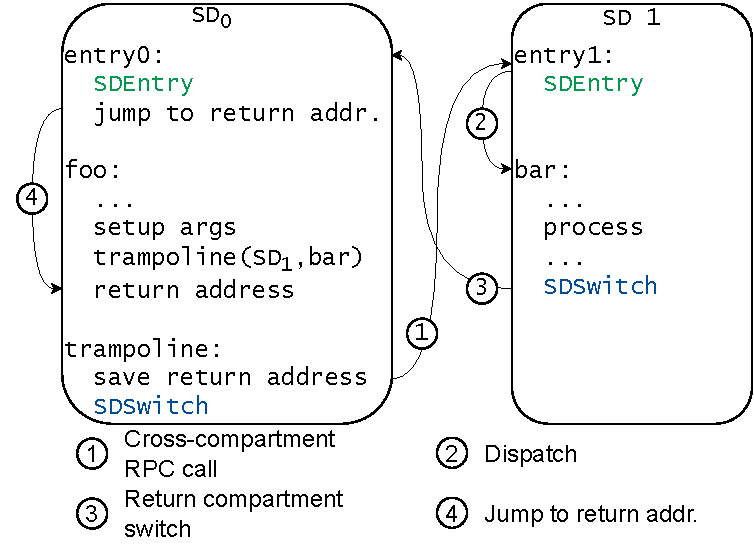
\includegraphics[width=0.7\linewidth]{media/seccells/sc_rpc.pdf}
  \caption{Cross-compartment procedure call in \seccells.}
  \label{fig:sc_rpc}
  %\Description[<short description>]{<long description>}
\end{figure}

Both forward and return edges on RPC-like cross-compartment 
calls use \sdswitch instructions, as illustrated in \autoref{fig:sc_rpc} 
where function \Code{foo} makes a cross-compartment call to \Code{bar}.
Arguments are passed in registers.
In this example, the caller uses a trampoline to hide its return address
before switching to \secdivx{1} (Step 1) and uses this address on the 
return path (Step 4).
\secdivx{0} is able to hide its calling address from \secdivx{1}, just
leaking the address of the generic trampoline.
Further, following the return switch to its entry point, \secdivx{0}
can read \rid to verify that the return is indeed from the called 
\secdiv, not any other.
On the other side, the callee (\secdivx{1}) can store its caller and
switch back to the caller's entry point on the backward edge.
If \secdivx{1} contains nested calls to other compartments, it
merely needs to remember its caller somewhere in its memory.
The dispatch (Step 2) secures the forward edge to \Code{bar} with call
gates.
While this example is secure, the flexibility of software allows other
calling patterns.

Context isolation requires the caller to save non-argument/return
registers to a state store before a \sdswitch and restore the same state
on the return edge.
The second step (context restore) is challenging since it
requires the \secdiv to find its state store without trusting any
register state, since the register state prior to the \sdswitch
persists.
We propose an array of per-\secdiv private \cell{}s as 
state stores, indexed by \sid.
The base of this array is easily constructed with
instruction pointer-relative instructions following an entry point.
Simple arithmetic involving the readable \sid register allows
a \secdiv to locate its state store, and consequently restore
the register state.
The latency of in-software context saving to memory is limited by 
the core's bandwidth to the L1 cache, the same as for any potential
hardware implementation.
Therefore, delegating this operation to software has no performance
impact.
Context switching also switches the stack pointer between 
per-compartment private stacks.

%-------------------------------
\subsection{Implementation}
\label{sec:seccells:impl}
%-------------------------------

Our implementation of \seccells augments and modifies the 
RocketChip~\cite{RocketChip} core and firmware.
An overview of the implementation is shown in 
\autoref{fig:seccell_arch}, with additions to the existing
processor highlighted in grey.
RISC-V provides the ideal, open platform for implementing fully-functional
prototypes of experimental architectures. 
\seccells permits a range of implementations for single and multi-core
processors containing in-order and/or out-of-order cores depending on the 
application's requirements: from firmware implementations on 
low-power embedded processors through hardware or 
microcode implementations on mobile, desktop, and server processors.
We discuss the trade-offs in detail in Appendix~\ref{app:impl_options}.
To match the RocketChip's simple, in-order pipeline, we implement 
access control and compartment switching in hardware within the pipeline 
and emulate the remaining instructions in firmware.

\seccells provides an alternate virtual memory mode, replacing 
SV-39 and SV-48.
We replace the core's MMU with a range-based TLB and a 
\ptable walker (replacing the traditional page-table walker).
We design the layout of the two-dimensional tables (\ptable and \gtable)
in memory to accelerate cell lookups and maximize 
spatial locality within the cache hierarchy when accessing permissions.
We add \sid and \rid to the core's Control-Status Registers (CSRs), 
and implement \sdswitch in the core pipeline.
The remaining instructions are implemented through hardware-assisted firmware 
by modifying OpenSBI~\cite{OpenSBI}.

The unified \ptable-\gtable in memory starts with a sorted
list of \cell descriptions, followed by the permissions held in the 
\ptable, and then the mappings for the \gtable.
% We don't have this layout any more
Appendix~\ref{app:ptable} shows the layout in detail.
Each \cell is described by the base and bound virtual addresses, 
the corresponding physical address base, and a single bit denoting
validity.
The sorted list of \cell{} descriptions allows the \ptable walker to
perform a binary search when looking for the cell which contains a particular
address, greatly accelerating lookups.
The row-major layout of the \ptable groups permissions for the same \secdiv
in contiguous cache lines, resulting in intra-cache line spatial locality for
permission lookups, and synergizing well with next-line prefetchers.
As a result, most MMU permission lookups are likely to be served by the L1 cache.
The unified \ptable-\gtable together occupies $\sim160kB$ to track permissions
to 1024 \cell{}s with 64 \secdiv{}s, equal to the memory used by leaf 
page-table entries to map $80$MB of data.

The range-based lookaside buffer holds a few \cell{} descriptions
and the corresponding permissions tagged by \sid.
The implementation of these structures is inspired by recent forays into 
range-based translation caches~\cite{0003BOBFP21midgard, YanLNB19, BasuGCHS13}, 
primarily aimed at tackling the limited reach of modern page-based translation 
lookaside buffers (TLBs).
Midgard~\cite{0003BOBFP21midgard} has shown that such lookaside buffers can 
sufficiently cover the working set of large applications with a 
few ($\sim$ 16) entries.

\seccells' userspace instructions are implemented through 
hardware-software co-design.
The \sdswitch instruction is implemented purely in hardware, and the
remaining permission-modifying instructions are emulated through firmware.
Additional hardware helpers, designed to aid operations trivially achieved
in hardware but costly in software, simplify and accelerate the emulation.
One notable operation is the lookup of the cell's index in the 
\ptable, which is common for all added instructions.
While a binary search in software is expensive, the MMU already holds this
information. 
We add an instruction, only accessible in RISC-V's machine mode and similar 
to the \Code{AT} instruction in ARMv8-A ISA~\cite{ARMAT}, to directly query the MMU.
We envision that higher performance processors with microcode sequencers
can implement these instructions in microcode, and
leave the investigation of the requirements of such an implementation
to future work.

%%%%%%%%%%%%%%%%%%%%%%%%%%%%%%%%
\section{Evaluation}
\label{sec:evaluation}
%%%%%%%%%%%%%%%%%%%%%%%%%%%%%%%%

In this section, we evaluate key metrics for \seccells' security and 
performance.
First, we show how \seccells provides security for the Browser described
in \autoref{sec:reqs}.
Second, we measure the latency of the \seccells' userspace instructions 
in microbenchmarks, particularly comparing compartment switching latency 
to related work.
We finally measure \seccells' performance for two representative workloads
highlighting the effect of range-based access control and
using userspace instructions for compartment switching and permissions
transfer.

\begin{table}
  \centering
  \caption{HW configuration of the \seccells prototype. }
  \begin{tabular}{l|c|c}
    \toprule
    Component             & \multicolumn{2}{c}{Configuration}                              \\
                          & Baseline                      & \seccells                      \\
    \midrule
    Core                  & \multicolumn{2}{c}{1 $\times$ Rocket, 6-stage, in-order}       \\
    L1 - D/I TLB          &  32-entry, fully-assoc.       & 16(D)/8(I)-entry, fully-assoc. \\
    L2 TLB                & 1024-entry, 4-way assoc.      & 32-entry, fully-assoc.         \\
    L1 D/I-cache          & \multicolumn{2}{c}{32KB, 8-way associative }                   \\
    L2 cache              & \multicolumn{2}{c}{16MB, 16-way associative}                   \\
    Main memory           & \multicolumn{2}{c}{DDR3, 800MHz, 1GB       }                   \\
    \bottomrule
  \end{tabular}
  \label{tab:testbench_cfg}
\end{table}



\begin{table}
  \centering
  \caption{FPGA resource utilization for SecureCells' MMU }
  \begin{tabular}{l | r  r  r | r  r  r}
    \toprule
                 & \multicolumn{3}{c|}{Traditional}  & \multicolumn{3}{c}{\seccells}  \\
                 & LUTs   & FFs   & SRAM             & LUTs & FFs   & SRAM            \\
    \midrule
    L1 ITLB      & 1915   & 1886  & 0                & 1529 &  869  & 0               \\
    L1 DTLB      & 2613   & 2048  & 0                & 1272 & 1903  & 0               \\
%   L2 TLB       & ----   & ----  & -                & ---- & ----  & -               \\
    L2 TLB + PTW & 5000   & 3428  & 18KiB            & 3826 & 4596  & 0               \\
%   Total(Core)  & ----   & ----  & -                & ---- & ----  & -               \\
    \midrule
    % \rowstyle{\bfseries}
    MMU Total    & 9528   & 7362  & 18KiB            & 6627 & 6200  & 0               \\
    \bottomrule
  \end{tabular}
  \label{tab:fpga_resource}
\end{table}

\paragraph{Testbench}
We ran the security evaluation on a QEMU implementation of \seccells,
which faithfully models its functional behavior, and the performance 
experiments on our hardware implementation of \seccells,
which uses cycle-accurate Register-Transfer Level (RTL) simulation to
accurately measure its timing behavior.
The core configuration, described in \autoref{tab:testbench_cfg}, 
resembles ARM's Cortex-A75. %~\cite{CortexA75}.
Our baseline is an identical core using a traditional page-based MMU
and TLBs instead of \seccells.
\autoref{tab:fpga_resource} shows the FPGA resource utilization for both the
baseline and \seccells MMUs.
\seccells' \ptable walker contains simpler logic than the baseline, 
as evidenced by the fewer LUTs required in the design.
Additionally, the much smaller range TLB eliminates the 18KiB block SRAM
required to store $1,024$ entries in the baseline L2 TLB.
We run our benchmarks on a seL4 kernel ported to use \seccells' 
memory protections. To evaluate realistic workloads on the seL4 kernel,
we faithfully ported core functionality of benchmarks, carefully limiting
system calls.

%-------------------------------
\subsection{Security Evaluation}
%-------------------------------

To evaluate \seccells' security claims, we test that a properly 
compartmentalized \seccells program prevents common attack vectors
for monolithic software.
We also include an in-depth analysis of \seccells' instruction semantics
afterwards.

\paragraph{Access Control}
We evaluate \seccells' access control on a mock Browser,
modeling the example described in \autoref{sec:reqs}.
The Browser contains a simple compiler Engine that generates code for
sandboxed WebApp applications.
The WebApp can allocate arrays, and read/write elements in the array through
get/set instructions.
We emulate a buggy Engine that generates vulnerable WebApp code lacking bounds 
checks on array accesses, allowing the WebApp arbitrary reads and writes.
With the monolithic Browser, an attacker WebApp could leak/modify the
Engine's data as well as that of a second sandboxed WebApp.
When compartmentalized with \seccells with the permissions shown in 
\autoref{fig:browser_eg}, illegal accesses by the attacker WebApp outside its
data \cell instead raise load/store access faults.
\seccells' access control also prevents arbitrary code injection by the WebApp
by preventing the WebApp from writing to either its or the Engine's code regions.

\paragraph{Context Isolation and Call Gates}
When uncompartmentalized, the WebApp can modify the Engine's stack enabling
control- and data-flow attacks like ROP~\cite{Shacham07}.
Using \seccells for separation, inter-compartment calls between the 
Engine and the WebApp are protected through call gates 
implementing context isolation (\autoref{sec:seccells:design:softmech}) including
stack switching.
\seccells successfully prevents the WebApp from accessing the Engine's stack.

\subsubsection{Formal Description and Analysis of \seccells' 
Userspace Instructions}
% \label{sub:instructions}

We define the semantics of \seccells' unprivileged instructions
in \autoref{fig:seccell_ops_formal} and discuss their corresponding
security checks below.

\paragraph{\sdswitch}
This instruction checks that the jump target is valid, and holds
an \sdentry instruction executable by the target \secdiv.
With the precondition that the caller \secdiv does not have
writable permission to any \cell executable by the target \secdiv,
\sdswitch guarantees compartment entry at previously defined entry 
points (helping implement call gates). 

\paragraph{\scprot}
This instruction checks that the target \cell is accessible by the
\secdiv, and the new permissions are a subset of the existing permissions.
After this instruction, the \secdiv is assured to have no more permissions
than before.

\paragraph{\scgrant, \screcv and \sctfer}
\scgrant checks that the granting \secdiv has permissions to the
\cell, and that the granted permissions are a subset of its existing
permissions.
\screcv, in turn, checks that the \secdiv is receiving permissions for a
valid cell, that the permissions were previously granted by the
specific \secdiv that the receiving \secdiv expects, and that the received
permissions are a subset of the permissions granted.
\sctfer includes the checks of both \scgrant and \scprot.
The granting and receiving \secdiv{}s must cooperate in order to
transfer permissions, and together finish with the same or fewer
permissions than they began with.

A correct compartment is defined to not grant or receive any permissions 
or invalidate cells that it is not required to grant as per a correct
compartmentalization policy.
Considering a set of compromised attacker \secdiv{}s and their permissions 
to \cell{}s and assuming that uncompromised compartments are correct,
\seccells guarantees that the attackers can neither gain any new permissions 
through any sequence of permission transfer instructions 
nor elevate the permissions of any uncompromised compartment.
Using \scgrant and \screcv instructions, the compromised compartments can
transfer permissions between themselves but those grants cannot include 
permissions which none of the attackers had initially.
The only way for the attackers to gain permissions is from
an uncompromised \secdiv either granting permissions to a \cell or from 
invalidating a private \cell which one of the attackers can validate with \screval.
The only way for the attackers to inject permissions is to have an
uncompromised \secdiv receive them.
By definition, uncompromised compartments will do neither of the above.
Once again, we stress on the importance of a correct compartmentalization
policy.
No mechanism, including \seccells, can protect against an insecure policy
where compartments transfer permissions from/to untrusted compartments
without proper validation.

\paragraph{\scinval} 
This instruction allows a \secdiv to invalidate a \cell to which
it has exclusive access, and to which no outstanding permission grants
exist.
The first condition can be true for a private region, or for one
which other \secdiv{}s have willingly dropped permissions.
Consequently, no other \secdiv will unwittingly lose permissions to
the invalidated \cell as a consequence of \scinval.
The second condition provides the assurance that no compartment can
regain permissions to the cell without executing \screval.

\paragraph{\screval} 
This instruction checks that the address corresponds to an existing 
\cell{} and that it is currently invalid. 
Due to the initial invalidity of the \cell, no \secdiv{}s could have
access to the cell to be revalidated.

\paragraph{\scexcl}
This instruction does not modify any permissions, only allowing a
\secdiv{} to check if it has exclusive access to a \cell{} to which
it already has access to.


%-------------------------------
\subsection{Performance Microbenchmarks}
%-------------------------------

% Comments on CHERI accounting:
% CHERI provided fine-grained overhead breakdown, which does not strictly
% conform to the
% categories in the aforementioned table. Therefore, we did need to figure
% out how to
% assign costs to categories. Therefore, the method is:
% Fixed costs       = kernel(receive trap) + kernel(exit kernel)
% context switching = caller + libcheri + kernel(clear non-arg registers)
% Switching cost    = Kernel SW operations
%       Switch	Ctx-switch	Other
%   42          42                       caller: Setup call, clear unused argument regs
%   34          34                       libcheri: Save callee-save regs, push call frame  
%   28  28                               kernel: Receive trap                               
%   79  79                               kernel: Validate CCall args.                       
%   41  41                               kernel: Push trusted stack, unseal CCall args.     
%   4   4                                kernel: Clear non-argument registers               
%   12  12                               kernel: Exit kernel                    
%   31  31                               kernel: Receive trap                               
%   7   7                                kernel: Validate return capability                 
%   4   4                                kernel: Clear non-return registers                  
%   41  41                               kernel: Pop trusted stack                          
%   7   7                                kernel: Exit kernel                                        
%   52          52                       libcheri: Pop call frame, restore regs.   
%   1           1                        caller: Back in caller                              
%--------------------------------------------------------------
%       254     129                      Total

\begin{table}
  \centering
  \caption{Compartment switching cost of \\various compartmentalization mechanisms.}
  \begin{threeparttable}
    \begin{tabular}{l | r | r | r | l | l}
      \toprule
                  & \multicolumn{3}{c|}{Round-trip Cycles}               & \multicolumn{2}{c}{CPU}   \\
                  & Switch         & \parbox[t]{1cm}{Context\\                                         
                                                     Saving}    & Total  & OoO\tnote{1} & Model      \\\midrule
      $lwC$       & \multicolumn{2}{c|}{$2 \times 6000$}        & 12000  & \checkmark   & SkyLake    \\
      seL4        & \multicolumn{2}{c|}{$2 \times 514 $}        & 1027   &              & RocketChip \\
      CHERI       & 254\tnote{2}   & 129\tnote{3}               & 425    &              & CHERI      \\
      ERIM        & $2 \times 99$  & Opt\tnote{5}               & 198    & \checkmark   & Xeon       \\
      XPC         & 82\tnote{4}    & Opt\tnote{5}               & 82     &              & RocketChip \\
      \seccells   & $2 \times 8$   & Opt\tnote{5}               & 16     &              & RocketChip \\
      \bottomrule
    \end{tabular}
    \begin{tablenotes}
      \item[1] Out-of-order CPUs incur higher pipeline serialization costs
      \item[2] In-kernel time
      \item[3] Userspace time (caller, libcheri)
      \item[4] XPC call + return + TLB miss
      \item[5] Optional, software-implemented context switch
    \end{tablenotes}
  \end{threeparttable}
  \label{tab:ipc}
\end{table}

\begin{table}[]
  \centering
  \caption{Cycles for emulating \seccells instructions.}
  \begin{tabular}{l | r | r | r | r}
    \toprule
    Instruction & \parbox[t]{0.7cm}{Trap\\ entry} 
                            & Dispatch  & Emulation & \parbox[t]{0.8cm}{Total \\Cycles} \\
    \midrule
    \scprot     & 79        &   32      &   33      & 144 \\
    \scinval    & 79        &   35      &   68      & 182 \\
    \screval    & 79        &   39      &   44      & 162 \\
    \screcv     & 79        &   54      &   69      & 202 \\
    \scgrant    & 79        &   52      &   63      & 194 \\
    \sctfer     & 79        &   61      &   62      & 202 \\
    \scexcl     & 79        &   57      &   67      & 203 \\
    \bottomrule
  \end{tabular}
  \label{tab:emulation}
\end{table}

First, we create microbenchmarks to measure the latency of each
userspace instruction introduced by \seccells, of which \sdswitch
is directly implemented in hardware, and the other instructions
are emulated in firmware.

In \autoref{tab:ipc}, we compare \seccells' compartment switching
cost with that of related mechanisms, particularly for a
round-trip cross-compartment call.
\seccells' userspace \sdswitch enables 8-cycle compartment switches,
with optional software context saving costs, which is more than $5\times$
faster than XPC's switch.
\sdswitch's latency consists of pipeline serialization (5 cycles), 
an instruction permission check (2 cycles) and a single cycle for the
targeted \sdentry instruction.
Of course, both XPC and \seccells would incur higher pipeline serialization
costs on an out-of-order core, putting \seccells on par with, or better than,
the MPK-based ERIM. 
Note that ERIM requires stringent code integrity and control-flow
integrity guarantees while \seccells does not impose any code requirements for
its compartmentalization guarantees.

All instructions other than \sdswitch and \sdentry are emulated by
the firmware, and therefore incur the costs of context saving, 
firmware entry and exit handlers, and dispatch to the correct
emulation function.
\autoref{tab:emulation} shows the latency of each instruction,
breaking down the cycles spent on each of the above overheads.
A microcode implementation of \seccells would allow the core to use 
internal registers for storage, eliminating the context switch, 
and directly lookup the microcode ROM to find the emulation 
microcode, eliminating dispatch.
Consequently, a microcode-based implementation would reduce 
\seccells' cost to that of the core emulation code only.

%-------------------------------
\subsection{Compartment Switching and Access Control}
%-------------------------------
To evaluate \seccells' practical performance, we create a simplified 
benchmark representative of a popular server workload, 
\Code{memcached}, accurately modelling the workload's memory access 
patterns across varying dataset sizes.
Our benchmark implements the core hashtable-based storage and the 
common query path loaded by an in-process load generator function
and omits system call-dependent features (networking, dynamic resizing),
and the global LRU list.
The benchmark isolates the data store from the vulnerable external interface
--- attackers might send malformed requests to trick the interface into directly
accessing the data store ---
by assigning them to separate \secdiv{}s.
The interface deserializes incoming requests, queries the data store
by switching compartments using \sdswitch, and serializes the
outgoing response.
For simplicity, this benchmark utilizes the migrating thread model.

\begin{figure}
  \centering
  \includegraphics[width=0.85\linewidth]{data/seccells/32ksim/mycached_full.pdf}
  \caption[\seccells performance comparison: \Code{memcached}]
          {Comparison of cycles-per-request,   
          cycles-per-instruction (CPI), and
          TLB miss rate
          while executing compartmentalized \Code{memcached} benchmark on 
          \seccells, compared to the uncompartmentalized version on RocketChip
          (lower is better).
          }
  \label{fig:mycached_cpi}
  %\Description[<short description>]{<long description>}
\end{figure}

Compartmentalizing the server allows us to measure the overheads
of frequent compartment switches, while varying the program's
dataset size allows us to compare \seccells' scalability.
We scale the dataset size by sweeping the number of fixed-size (64B)
entries stored in the data store, all of which are accessed randomly
by the load generator.
We compare the compartmentalized server running on \seccells'
implementation to an uncompartmentalized server running on
an unmodified RocketChip core by measuring the average count of
instructions retired and cycles used to process each request.
To compare against another emerging compartmentalization architecture,
we also conservatively model CHERI's performance on this benchmark,
adding the costs of supervisor-mediated compartment
switches with hardware support, as reported in the 
CHERI paper~\cite{WatsonWNMACDDGL15}.
We model each compartment switch as 191 instructions requiring 254 cycles,
excluding the costs of context switching and
ignoring other microarchitectural overheads.
In \autoref{fig:mycached_cpi}, we plot the average per-request 
cycle count and the cycles-per-instruction (CPI) for the server.

\seccells implements fast compartment switching, and 
the cost of switching to and from the data store compartment
for each request (16 cycles) is minuscule ($< 3\%$) compared to the
request processing time (minimum 532 cycles).
Consequently, \seccells' performance closely tracks that of 
the baseline even for small dataset sizes.
In contrast, CHERI's compartment switching overwhelms the
request processing time, only approaching the baseline's
performance for large dataset sizes.
While CHERI's performance for compartmentalization compares
favorably to that of traditional OS-based isolation 
techniques, it offers unacceptable overheads for finer, 
function-granularity compartmentalization (up to 95.5\%).

The CPI graph highlights the baseline system's limited TLB 
reach.
As the dataset exceeds the TLB reach of 4MB, the baseline starts
to encounter TLB misses on accesses to the data store.
Consequently, the baseline CPI starts to degrade compared to
\seccells, and only worsens as the dataset increases past the
CPU's last-level cache capacity.
In contrast, \seccells' range-based lookaside buffer comfortably
scales to large datasets, allowing the \Code{memcached} server to
serve requests 9.3\% faster for a 32MB dataset.
 
%-------------------------------
\subsection{Compartmentalized pipeline}
%-------------------------------

\begin{figure}
  \centering
  \includegraphics[width=0.85\linewidth]{data/seccells/network_1ktlb_sim/nfv_full.pdf}
  \caption[\seccells performance comparison: Network function]
          {Packet processing cycles-per-byte comparison.}
  \label{fig:nfv_cpb}
  %\Description[<short description>]{<long description>}
\end{figure}

To illustrate \seccells' zero-copy permission transfer performance,
we implement the virtual network function pipeline presented in
\autoref{fig:dataflow_app}.
The Driver stage generates a ``packet'' by writing a UDP/IP packet
of varying length into a packet buffer, whereas 
the Firewall and NAT read and modify the IP and UDP headers
respectively, but ignore the packet's payload.

Representing the ideal performance target,  we include the
``uncompartmentalized'' configuration that passes the packet by 
reference, incurring no overheads for data transfer.
The second configuration, ``compartmentalized-copy'', 
compartmentalizes pipeline stages and uses shared buffers to transfer
packets by copy.
The third, zero-copy ``\seccells ZC''  configuration isolates
stages, and uses userspace instructions to transfer 
access permissions to packets, each of which occupies a
different \cell{}.
Finally, the ``\seccells ZC-$\mu$code'' configuration models the 
possible performance of a microcode implementation of \seccells' 
dataflow instructions by mitigating trapping overheads
to the firmware and dispatch.
This model is conservative, ignoring possible optimizations from
parallelizing checks in microcode.

In \autoref{fig:nfv_cpb}, we plot the average number of cycles
required by the benchmark to process a byte of a packet
as the packet size grows.
Fixed costs, such as a function call, compartment switch or 
permission transfer, have diminishing impacts as the packet size grows.
The costs for generating and copying the packet, however, grows
linearly with packet size, and add a constant vertical offset in the
graph.
The ``compartmentalized-copy'' configuration incurs additional costs over the
uncompartmentalized baseline due to 
compartment switches (4.4\% for small packets) and packet copy (51.1\%).
The ``\seccells ZC'' configuration trades-off linearly-growing 
packet copying costs with fixed-cost permission transfers and
(in)validations.
While the $\sim250$-cycle average latency of \seccells' 
permission-modifying instructions causes a massive 199\% overhead
for the smallest packets, this fixed cost quickly gets amortized
for larger packets.
Indeed, this configuration overtakes the ``compartmentalized-copy'' configuration
for 600B packets and above, and approaches the performance
of the uncompartmentalized configuration (2.0\% overhead) for
16kB packets.
Finally, the ``\seccells ZC-$\mu$code'' configuration highlights \seccells'
performance potential, with (average) 69-cycle operations for 
transferring permissions which lowers the break-even threshold to
200B packets.

%%%%%%%%%%%%%%%%%%%%%%%%%%%%%%%%
\section{Related Work}
\label{sec:related}
%%%%%%%%%%%%%%%%%%%%%%%%%%%%%%%%

A variety of compartmentalization techniques exist, both in software and
leveraging hardware, targeting differing goals and with consequently
different designs.

Attacks often target specific, sensitive data for 
leakage or corruption (e.g., keys or flags).
Consequently, various proposals such as IMIX~\cite{FrassettoJLS18},
ERIM~\cite{ERIMOberwagner19}, and MemSentry~\cite{KoningCBGA17} introduced 
mechanisms to specifically protect 
such data from untrusted or unsafe code.
However, these mechanisms fail to apply to more generic scenarios,
with more than two compartments, per-compartment sensitive or private
data, and non-hierarchical trust models.
COde-centric memory DOMains~\cite{VilanovaBNEV14} proposed an architecture
where the instruction pointer identifies the running compartment, in a bid
to isolate untrusted libraries.
However, this proposal is unable to support the extensive code sharing 
in modern programs, including shared libraries like \Code{libc}.

Compatibility with existing systems brings immediate security benefits.
By mapping the same physical pages across separate per-compartment page 
tables with different permissions, the existing virtual memory implementation
can mimic intra-address space compartmentalization.
Typically, such mechanisms require costly supervisor intervention to
switch compartments limiting the temporal granularity of compartmentalization.
SMV~\cite{HsuHEP16} introduced an API for creating intra-address space
memory views, but relied on the supervisor for compartment transitions.
Light-Weight Contexts~($lwC$)~\cite{LittonVE0BD16} proposed a new OS 
abstraction enabling a fast-path in the supervisor for compartment switching,
essentially eliminating overheads from unnecessary tasks such as scheduling.
$lwC$ successfully reduces the cost of a compartment switch from 4 to 2$\mu$s,
but remains an order of magnitude away from nanosecond-scale switching.
Hodor~\cite{HedayatiGJCSSM19Hodor} uses the VMFUNC instruction, 
introduced for virtual machines, to instead switch page tables in a few 
hundred cycles, eliminating supervisor overheads but consequently
inherits the additional costs of two-dimensional page table walks.
LOTRx86~\cite{LeeSK18} repurposed unused x86 rings to introduce a
privileged userspace for storing sensitive data.
XPC~\cite{DuHXZC19XPC} prioritized software compatibility, choosing to
accelerate the remote-procedure call (RPC) interface used for 
process-based compartmentalization with new userspace instructions.
To achieve this goal, XPC cores track a complicated system of metadata across the
cores and memory, storing a list of compartments, entry points, valid
caller-callee pairs, and a caller stack.
XPC is secure, performant, and can allow exclusive access to a single
data memory range at almost zero cost.
However, XPC requires additional caches for dedicated storage of its
metadata, does not allow permissions to be transferred, and requires
hardware to implement features cheaply implementable in software 
(e.g., call stacks), and cannot support non-RPC like compartment
switches.
With page table-based virtual memory, such proposals all inevitably suffer 
from the scalability limitations of modern TLBs~\cite{PhamVJB12, YanLNB19, 
BasuGCHS13}.

Existing architectures have introduced features for intra-address
space isolation, e.g., Intel's MPK and ARM's MTE extensions,
with fast compartment switching ($<100$ cycles) in the common case.
These extensions enforce additional permissions, but
are insecure under stronger threat models due to designs which
prioritize compatibility with existing processors.
MPK, for example, is defeated by arbitrary code injection.
ERIM~\cite{ERIMOberwagner19} requires complicated code scanning to
prevent code injection, and Donky~\cite{SchrammelWSS0MG20Donky} requires 
hardware modifications to introduce an additional trusted privilege level 
within userspace.
Since neither ERIM nor Donky validates code accesses, an attacker
targeting cross-compartment code injection need not make the
malicious code executable for the target before tricking the target 
into executing this code.
Memory keys also architecturally limit the number of memory regions for 
which permissions can be efficiently tracked, leaving no room for future 
microarchitectural advances to improve code performance.
These systems also inherit the TLB-reach issues of modern TLBs.

Range-based permission tracking tackling the TLB-reach issue 
appeared in Mondrian Memory Protection (MMP)~\cite{WitchelCA02MMP}.
MMP proposed a virtual memory architecture tracking segment-based 
permissions for compartments within an address space, 
simulating zero-copy for networking through redundant mappings for
packet buffers with different, static permissions.
MMP only implements access permission checks in hardware, 
delegating other operations, including compartment switches, 
to the supervisor, precluding high-performance applications.
MMP also uses different permissions tables for each compartment,
reading duplicated range boundaries on each switch.

CHERI refers to hardware-enforced memory capabilities~\cite{WoodruffWCMADLNNR14}, 
and an eponymous compartmentalization mechanism reusing the same 
capabilities~\cite{WatsonWNMACDDGL15}.
The original proposal for memory capabilities offers a practical
mechanism to mitigate spatial safety bugs,
restricting the ability of pointers to access memory beyond bounds.
We recognize that CHERI's capabilities can prevent memory corruption within
a compartment, motivating integration  with \seccells
to together improve security.
CHERI compartmentalization encapsulates capabilities to a compartment's
code and data, relying on costly supervisor-mediated compartment switches.
CHERI lacks auditability since capabilities are spread throughout
memory, and a bug resulting in a capability being leaked cannot be cheaply
detected and fixed.
CHERI's switching costs are not security-proportional, lacking the
ability to skip context switching costs when acceptable.
Finally, CHERI's permissions are built on traditional page-based translations,
and inherit TLB limitations.
Nonetheless, CHERI allows more granular per-object capabilities as compared
to \seccells' per-VMA permissions.
% The distributed nature of permissions also means that a compartment
% can never be assured of exclusive access to a memory region and also
% implies a memory overhead
% proportional to the number of capabilities stored in program memory.

Along with mechanisms, policy research is equally important.
Researchers have attempted to formalize a compartment program's 
guarantees~\cite{JuglaretHAEP16}, determine the scope of access following
permission transfers under the take-grant model~\cite{LiptonS77},
automatically infer isolation policies from 
programs~\cite{RoesslerAPMPKPB21,KirthDCLDGNVF22,VasilakisKRDDS17},
provide hints to programmers on isolation boundaries based on
automated analysis~\cite{GudkaWACDLMNR15}, and
reason about what guarantees remain when one or more compartments are
compromised~\cite{AbateABEFHLPST18}. 

%%%%%%%%%%%%%%%%%%%%
\section{Discussion}
\label{sec:seccells:discussion}
%%%%%%%%%%%%%%%%%%%%

\paragraph{Legacy program/OS support}
\seccells is compatible with existing pre-emptive operating systems which 
already separate architecture-specific memory management code.
\seccells also supports page-based memory management (demand paging, swapping)
when integrated with upcoming intermediate-address space memory 
architectures~\cite{ZhangSRL10,0003BOBFP21midgard}.
Since \seccells preserves the VMA-based view of virtual memory, 
an OS can present a legacy userspace environment for existing monolithic
applications by allocating a single compartment in the \ptable.
Legacy applications will also benefit from \seccells' improved 
TLB-reach with range-based address translations.

\paragraph{Adopting \seccells}
\seccells faces the daunting task of changes across the software and 
hardware stack.
Nonetheless, library and compiler support for software development
can greatly aid developer adoption.
%To evaluate our benchmarks, 
We developed a prototype library
(\Code{scthreads})
to support compartments with isolated contexts, and envision that
most software can be ported through compilation with a
\seccells-compatible C/C++ library.
We compartmentalized the example Browser ($\sim$1kLoC), 
initially developed and tested on an \Code{x86} machine, 
in approximately two additional days.
Software such as browsers desiring the full benefits of compartmentalization
will still require rewriting (to refactor monolithic code into compartments).
\seccells' userspace instructions map to common compartmentalized
applications' operations, evidenced by strong parallels between
\seccells' instructions and APIs in related mechanisms or 
language-level operations in compartmentalization
frameworks (\autoref{tab:api_mapping}).
This mapping will simplify porting existing compartmentalized
applications, such as Nginx-lwC~\cite{LittonVE0BD16}, to run on \seccells
by replacing existing operations with the \seccells equivalent 
(e.g., substitute \sdswitch in place of \Code{lwSwitch}).
Existing software compartmentalization libraries and compilers~\cite{HsuHEP16}
can also use \seccells as a backing mechanism.
%
For example, consider a \seccells backend for the LitterBox sandbox,
used by the compartmentalizing compiler Enclosures~\cite{GhosnKPLB21}
to isolate untrusted Go libraries, improving performance and security over
the existing Intel VT-x and MPK backends respectively.
Enclosure switching (\Code{Prolog} and \Code{Epilog}) map to \sdswitch
instructions whereas data movement (\Code{transfer}) maps to a 
\sctfer-\screcv pair.

\begin{table}[h]
  \caption{Mapping \seccells instructions to related mechanisms, libraries and language features.}
  \begin{threeparttable}
    \begin{tabularx}{\columnwidth}{p{1.4cm} | >{\raggedright\arraybackslash}X}
    \toprule
      Instruction & Analogous API \\
    \midrule
      \sdswitch  &                                                                                    \Code{dcall}~\tnote{3},                \Code{CCall/CReturn}~\tnote{4}, \Code{Prolog/Epilog}~\tnote{5}, \Code{lwSwitch}~\tnote{6}  \\ %\midrule
      \scprot    &                  \Code{mprotect}\tnote{1},          \Code{mpk_mprotect}~\tnote{2}, \Code{dk_mprotect}~\tnote{3},          \Code{CAndPerm}~\tnote{4}                                                                  \\ %\midrule
      \scinval   &                  \Code{munmap}\tnote{1},            \Code{mpk_free}~\tnote{2},     \Code{dk_munmap}~\tnote{3}                                                                                                        \\ %\midrule
      \screval   &                  \Code{mmap}\tnote{1},              \Code{mpk_mmap}~\tnote{2},     \Code{dk_mmap}~\tnote{3}                                                                                                          \\ %\midrule
      \scgrant \screcv \sctfer &    \Code{mmap(MAP_PRIVATE)}\tnote{1},                                \Code{dk_domain_assign_key}~\tnote{3},                                  \Code{Transfer}~\tnote{5},     \Code{lwOverlay}~\tnote{6} \\ %\midrule
      % \scexcl    & N/A                                                                                                                                                                                                                  \\
    \bottomrule
    \end{tabularx}
    \begin{multicols}{2}
    \begin{tablenotes}
      \item[1] Linux processes
      \item[2] \Code{libmpk}~\cite{ParkLXMK19}
      \item[3] Donky~\cite{SchrammelWSS0MG20Donky}
      \item[4] CHERI~\cite{WatsonWNMACDDGL15,WoodruffWCMADLNNR14}
      \item[5] Enclosures~\cite{GhosnKPLB21}
      \item[6] lwC~\cite{LittonVE0BD16}
    \end{tablenotes}
  \end{multicols}
  \end{threeparttable}
  \label{tab:api_mapping}
\end{table}

% Possibly remove for resubmission
% Bring back for camera ready
\paragraph{System call semantics with \seccells}
Recent work~\cite{ConnorMSS20} has demonstrated that the Linux system call
interface can be used to compromise userspace compartmentalization.
Modifications of the syscall interface, such as those proposed in 
Jenny~\cite{schrammel2022jenny}, are orthogonal to the compartmentalization
mechanism and can be applied to \seccells.
We leave a systematic evaluation of kernel performance and 
system call semantics with \seccells to future work.

\paragraph{Advantages for microkernels and system calls}
Fast compartmentalization is the key objective for practical microkernel
operating systems.
By running the OS kernel and drivers in \secdiv{}s, \seccells improves over
a modern microkernel's switching time by two orders of magnitude.
Similarly, userspace programs can benefit from significantly faster system
calls if the kernel is assigned a compartment within each program's address
space.
Essentially, the costly system call entrances can be replaced by cheaper
\sdswitch instructions into the kernel.  

\paragraph{Speculative-execution attacks (SEA)}
We consider the threat of speculative side-channel attacks like 
Spectre~\cite{KocherHFGGHHLM019} in \seccells' design, despite 
omitting such attacks from our attacker model.
\seccells{} introduces additional mechanisms for changing an executing
thread's permissions, through userspace compartment switching and
permission transfers.
Fault-based attacks like Meltdown~\cite{lipp18sec} must be prevented in
implementations by preventing faulting loads from accessing memory or
forwarding their data to subsequent instructions~\cite{WeisseNLWK19}.

\seccells does not mitigate existing SEA, but takes care
not to introduce vulnerabilities.
\seccells specifies that userspace instructions are serializing, 
precluding speculative permission changes.
An attacker cannot, for example, speculatively switch to a victim
\secdiv using an \sdswitch following a long-latency branch and read 
the victim's private data using the victim's permissions.
\seccells' permission transfer instructions are atomic, preventing visibility 
or exploitation of any intermediate permission state.
An attacker \secdiv cannot, for example, drop permissions for a \cell
using \scprot while transferring the same permissions using \sctfer in parallel.
Our firmware (and future microcode) implementation use load-linked 
store-conditional atomic operations commonly available across architectures
to ensure atomicity.


\seccells' access control limits the leakage scope of 
Spectre attacks to a compartment's accessible \cell{}s, 
weakening SEA.
\seccells allows the pipeline to speculate as usual within a compartment's 
execution, and speculative accesses are also subject to access control 
by the MMU and cannot illegally access any \cell.
Access control, therefore, also limits the leakage potential of existing
Spectre gadgets.
Whereas a Spectre gadget on a traditional processor can address and
access any user memory in the process' address space, the same Spectre
gadget can only access memory within the compartment's \cell{}s.
\seccells also limits the code (speculatively) executable within a compartment,
further restricting the availability of Spectre gadgets.


%%%%%%%%%%%%%%%%%%%%%%%%%%%%%%%%
\section{Conclusion}
%%%%%%%%%%%%%%%%%%%%%%%%%%%%%%%%

Compartmentalization requires labor-intensive code restructuring, 
deterring developers from adopting piecemeal solutions which provide
partial protection or which cripple performance.
This chapter introduces \seccells, a secure, flexible and 
performance-focused compartmentalization architecture to
underpin future software compartmentalization efforts.
Further work is required, for 
scaling our FPGA prototype to an out-of-order, multicore processor, 
investigating implementations of higher-level abstractions 
on \seccells' mechanisms,
developing software conventions to develop correctly
compartmentalized programs for \seccells, 
and to improve OS support for the architecture.

Nevertheless, \seccells enables practical, effective, and efficient
compartmentalization by tackling 
the core architectural requirements for a mechanism.
\seccells strictly enforces access controls and protects permissions
from corruption, while supporting secure 8-cycle compartment switching.
\seccells constrains inter-compartment control flow to respect
call gates, protecting these interfaces from fault propagation.
\seccells is also an enabler for data processing pipelines
with userspace zero-copy data transfers.
\seccells remains flexible, eschewing policy-specific specializations.
We have published the \seccells prototype, benchmarks
and supporting infrastructure
at \url{https://www.hexhive.epfl.ch/securecells}.
